\section{Single Source Shortest Path}

\begin{frame}
  \begin{center}
    {\bf Part I - Djikstra (Shortest Path)}
  \end{center}
\end{frame}

\subsection{Definitions}
\begin{frame}
  \frametitle{SSSP: Single Source Shortest Path}
  \begin{block}{Problem Definition}
    In a graph $G(V,E)$, find the path from vertex $v_s$ (source) to vertex $v_t$ (target), with {\bf minimum sum of weights}.
  \end{block}\bigskip

  \begin{itemize}
  \item If the graph is {\bf unweighted} (every weight is equal), use Breadth First Search (BFS).\medskip

  \item Start BFS on node $v_s$;\medskip

  \item BFS visits all vertices by order of distance, and reach $v_t$ with minimum steps;
  \end{itemize}
\end{frame}

\begin{frame}[fragile]
  \frametitle{BFS Implementation for SSSP}

{\smaller
\begin{exampleblock}{}
\begin{verbatim}
vector <int> p;                          // parent list
vector <int> dist(V,100*V); dist[s] = 0; // dist matrix
queue  <int> q;           q.push(s);

while (!q.empty()) {
   int u = q.front(); q.pop();
   for (int j = 0; j < AdjList[u].size(); j++) {
      int v = AdjList[u][j];
      if (dist[v] > V) {                 // not visited
         dist[v] = dist[u] + 1;
         p[v] = u; q.push(v); }}}

void printPath(u) {                      // path from (u)
   if (u == s) { cout << s; return; }
   printPath(p[u]); cout << " " << u; }
\end{verbatim}
\end{exampleblock}
}
\end{frame}

\begin{frame}
  \frametitle{BFS does not work with weighted graphs}

  \begin{block}{}
    BFS is simple and fast when the graph is {\bf unweighted}.\bigskip

    But when the graph has weights, BFS gives you {\bf wrong answer}.
  \end{block}

  \medskip

  \begin{center}
    \begin{tikzpicture}[transform shape,label/.style={thin, draw=black, align=center,fill=white,font=\smaller},scale=1.1]
      \node[vertex] (a) at (0,0) {t};
      \node[vertex] (b) at (1,1) {};
      \node[vertex] (c) at (2,0) {};
      \node[vertex] (d) at (1,-1) {e};
      \node[red vertex] (e) at (-1,-1) {s};
      \draw[edge] (a) -- node[label] {$1$} (b);
      \draw[edge] (b) -- node[label] {$2$} (c);
      \draw[edge] (a) -- node[label] {$4$} (c);
      \draw[red edge] (a) -- node[label] {$2$} (d);
      \draw[edge] (c) -- node[label] {$1$} (d);
      \draw[red edge] (a) -- node[label] {$6$} (e);
      \draw[black edge] (d) -- node[label] {$9$} (e);
    \end{tikzpicture}
  \end{center}

  \bigskip

  \begin{itemize}
  \item BFS shortest path: $s \rightarrow e$ (1 edge, cost 9)
  \item Real shortest path: $s \rightarrow t \rightarrow e$ (2 edges, cost 8)
  \end{itemize}
\end{frame}

\subsection{Dijkstra Algorithm}
\begin{frame}
  \frametitle{SSSP on weighted graphs: Dijkstra's Algorithm}
  \begin{block}{Basic Idea: Greedy Graph Search}
    Always visit the vertex with {\bf minimal total distance} from the source vertice.
  \end{block}\bigskip

  \begin{itemize}
  \item There are many different implementations;
  \begin{itemize}
    \item (The original paper did not include a specific implementation!)
  \end{itemize}\bigskip

  \item Simple implementation: replace the BFS {\bf queue} with a {\bf Priority Queue}:
  \begin{itemize}
    \item The priority queue sorts the edges by total distance from source;
  \end{itemize}\bigskip

  \item Note: Lazy Deletion Optimization
  \begin{itemize}
    \item C++ STL priority queue has large cost to deleting/updating edges;
    \item To avoid this cost, we do not delete edges (but skip them if necessary);
  \end{itemize}
  \end{itemize}

\end{frame}

\begin{frame}[fragile]
  \frametitle{Dijkstra's Algorithm Implementation Example}

  This implementation uses {\bf Lazy Deletion} to reduce the number of deletions in the priority queue;

  {\smaller
    \begin{exampleblock}{}
\begin{verbatim}
typedef pair<int,int> ii;           // <distance, to_vertex>
priority_queue<ii, vector<ii>, greater<ii>> pq;
pq.push({0,s});

while (!pq.empty()) {
  auto [d, u] = pq.top(); pq.pop(); // shortest unvisited u
  if (d > dist[u]) continue;        // skip edges that don't improve the path
  for (auto &[v, w] : AdjList[u]) { // all edges from u
    if (dist[u] + w >= dist[v]) continue;
       // new edge does not improve solution, skip
    dist[v] = dist[u] + w           // update distance
    pq.push({dist[v], v})           // enqueue better pair
  }
\end{verbatim}
    \end{exampleblock}}
\end{frame}

\begin{frame}[fragile]{Dijkstra with Lazy deletion: Simulation}
  Dijkstra visits vertices: 2, 1, 3, 0, 4; in order
  \begin{columns}[T]
    \column{0.6\textwidth}
    \begin{center}
      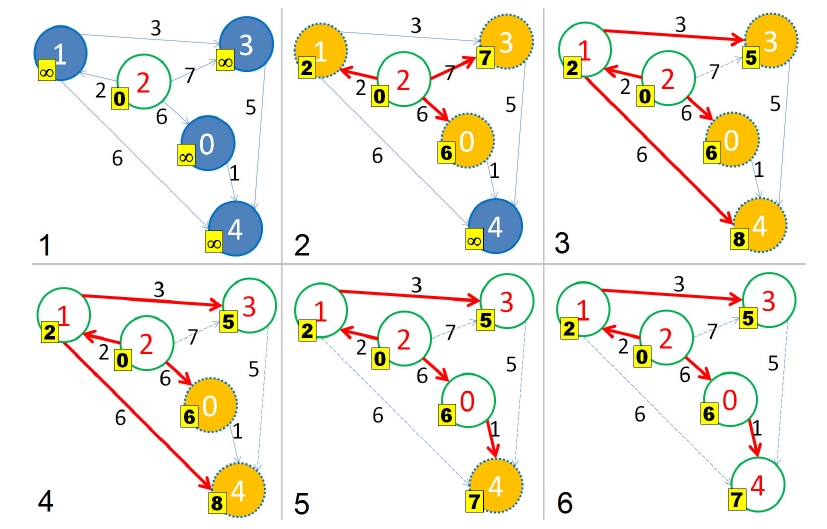
\includegraphics[width=.9\textwidth]{../img/dijkstra_halim}
      \ppagenote{Dijkstra Image from "Competitive Programming 3", Steven Halim}
    \end{center}
    \column{.4\textwidth}
\begin{verbatim}
 PQ:
\end{verbatim}
  \end{columns}
\end{frame}

\subsection{Problem Example}

\begin{frame}{SSSP and Programming Challenges}
  \begin{itemize}
    \item Use the {\bf Practice Problem} to train the implementation of Djikstra;\bigskip

    \item In Programming Challenges, a big part of the problem is to build the correct graph;\bigskip

    \item Think about the correct {\bf vertices, edges and weights} from the input data;
  \end{itemize}
\end{frame}

\begin{frame}
  \frametitle{Example Problem -- Full Tank}
  \begin{block}{Problem Summary}
    Find the {\bf cheapest} path from city $S$ to city $T$. Consider the following:

    \begin{itemize}
      \item To go from $v_i$ to $v_j$ requires $E_{i,j}$ {\bf liters of fuel};
      \item {\bf We must buy fuel}: The price of fuel in city $v_i$ is $p_i$;
      \item Your car has maximum capacity $c$;
    \end{itemize}
  \end{block}

  \begin{center}
    \begin{tikzpicture}[transform shape,label/.style={thin, draw=black, align=center,fill=white,font=\smaller},scale=1.1]
      \node[red vertex] (s) at (0,0) {s:4};
      \node[vertex] (0) at (2,1) {a:6};
      \node[vertex] (1) at (4,1) {b:1};
      \node[vertex] (e) at (6,0) {t:0};
      \draw[edge] (s) -- node[label] {$5$} (e);
      \draw[edge] (s) -- node[label] {$1$} (0);
      \draw[edge] (0) -- node[label] {$1$} (1);
      \draw[edge] (1) -- node[label] {$5$} (e);
    \end{tikzpicture}
  \end{center}

  \begin{itemize}
    \item Path: $s\to t$: Buy 10 liters at $s$, cost: 20
    \item Path: $s\to a\to b\to t$:
    \begin{itemize}
      \item Buy 4 liters at $s$, 10 liters at $b$, cost: 9
    \end{itemize}
    \item {\bf QUIZ}: What is the correct graph structure to solve this problem?
  \end{itemize}
\end{frame}

\begin{frame}
  \frametitle{Example Problem -- Full Tank: Building the Graph}

    \begin{center}
      \begin{tikzpicture}[transform shape,label/.style={thin, draw=black, align=center,fill=white,font=\smaller},scale=1.1]
        \node[red vertex] (s) at (0,0) {s:4};
        \node[vertex] (0) at (2,1) {a:6};
        \node[vertex] (1) at (4,1) {b:1};
        \node[vertex] (e) at (6,0) {t:0};
        \draw[edge] (s) -- node[label] {$5$} (e);
        \draw[edge] (s) -- node[label] {$1$} (0);
        \draw[edge] (0) -- node[label] {$1$} (1);
      \draw[edge] (1) -- node[label] {$5$} (e);
      \end{tikzpicture}
    \end{center}

    \begin{itemize}
      \item Transform vertex $v_i$ into a set of vertices $v_{i,f}$: $v_{i,0}, v_{i,1}, \ldots, v_{i,c}$;
      \begin{itemize}
        \item This represents the car at $v_i$ with $f$ fuel left;
      \end{itemize}
      \item An edge exists between $v_{i,k}$ and $v_{i,k+1}$ with cost $p_i$;
      \begin{itemize}
        \item This represents adding fuel to the car.
      \end{itemize}
      \item An edge exists between $v_{i,k}$ and $v_{j,k-w_{i,j}}$ {\bf if}:
      \begin{itemize}
        \item exists an edge $v_i \to v_j$ in the original graph with cost $w_{i,j}$
        \item $k-w_{i,j} \geq 0$;
        \item This represents the car has enough fuel to go from i to j
      \end{itemize}
      \item Now we can do Dijkstra in the modified graph;
      \item Note the new graph has $V\times C$ vertices and $E\times C$ edges;
    \end{itemize}
\end{frame}

\begin{frame}
  \frametitle{Example Problem -- Full Tank: Simulation of Graph Transformation}

    \begin{center}
      \begin{tikzpicture}[transform shape,label/.style={thin, draw=black, align=center,fill=white,font=\smaller},scale=1.1]
        \node[red vertex] (s) at (0,0) {s:4};
        \node[vertex] (0) at (2,1) {a:6};
        \node[vertex] (1) at (4,1) {b:1};
        \node[vertex] (e) at (6,0) {t:0};
        \draw[edge] (s) -- node[label] {$5$} (e);
        \draw[edge] (s) -- node[label] {$1$} (0);
        \draw[edge] (0) -- node[label] {$1$} (1);
      \draw[edge] (1) -- node[label] {$5$} (e);
      \end{tikzpicture}
    \end{center}
    \vspace{10cm}

\end{frame}
